\documentclass[tikz,border=10pt]{standalone}
\usepackage{ctex} % 如需中文支持
\usetikzlibrary{calc}

\begin{document}
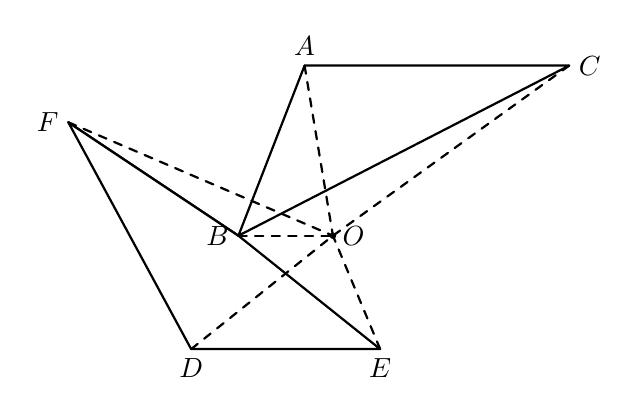
\begin{tikzpicture}[scale=1.2, >=stealth, line join=round, line cap=round]
    % --- 1. 定义核心坐标点 ---
    % 中心参考点 O
    \coordinate (O) at (0,0);
    
    % 上方图形顶点 (A, B, C)
    \coordinate (B) at (-1,0); 
    \coordinate (A) at (-0.3,1.8);
    \coordinate (C) at (2.5,1.8);
    
    % 下方/侧方图形顶点 (D, E, F)
    \coordinate (D) at (-1.5,-1.2);
    \coordinate (E) at (0.5,-1.2);
    \coordinate (F) at (-2.8,1.2);

    % --- 2. 绘制实线部分 (图形轮廓) ---
    % 上方区域
    \draw[thick] (A) -- (C) -- (B) -- cycle;
    
    % 下方/左侧区域
    \draw[thick] (F) -- (D) -- (E) -- (B) -- cycle;
    \draw[thick] (F) -- (B);

    % --- 3. 绘制虚线部分 (辅助线与内部连接) ---
    \draw[dashed, thick] (A) -- (O);
    \draw[dashed, thick] (C) -- (O);
    \draw[dashed, thick] (B) -- (O);
    \draw[dashed, thick] (D) -- (O);
    \draw[dashed, thick] (E) -- (O);
    \draw[dashed, thick] (F) -- (O);

    % --- 4. 标注文本标签 ---
    % 使用 pos 或 偏移手动调整位置，确保不被线段遮挡
    \node[above] at (A) {$A$};
    \node[left]  at (B) {$B$};
    \node[right] at (C) {$C$};
    \node[below] at (D) {$D$};
    \node[below] at (E) {$E$};
    \node[left]  at (F) {$F$};
    \node[right] at (O) {$O$};

    % 可选：在 O 点打一个小点
    \fill (O) circle (1pt);
\end{tikzpicture}
\end{document}